\section{Results}\label{sec:results}

The system was tested with 82 images that contained banknotes in the most common conditions, such as different perspective views, cluttered environments, multiple banknotes per image and partially occluded banknotes. With the proper configuration, the system successfully recognize all test images. In \cref{fig:recognition-clutter,fig:recognition-perspective-distortion,fig:recognition-partially-occluded-banknotes,fig:recognition-overlapping-banknotes} are shown some representative results of the implemented banknote recognition system.

\begin{figure}[H]
	\centering
	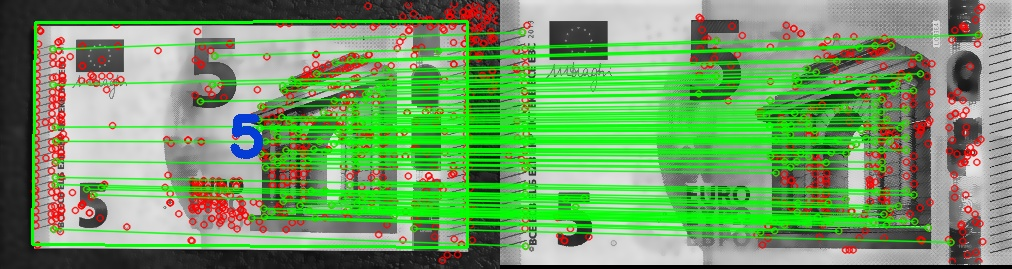
\includegraphics[width=0.498\textwidth]{notes-recognition/5__(5).jpg___SIFT-Detector_SIFT-Extractor_BF-Matcher_lowQualityImageDB_globalMatch__inliersMatches__0}\hfill
	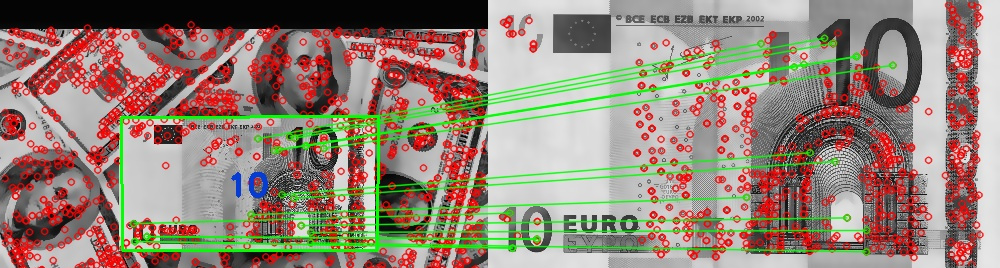
\includegraphics[width=0.498\textwidth]{notes-recognition/10__(9).jpeg___SIFT-Detector_SIFT-Extractor_BF-Matcher_lowQualityImageDB_globalMatch__inliersMatches__0}
	\caption{Detection of a banknote in an ideal perspective view with and without background clutter (using SIFT detector, SIFT descriptors and BFMatcher)}
	\label{fig:recognition-clutter}
\end{figure}

\begin{figure}[H]
	\centering
	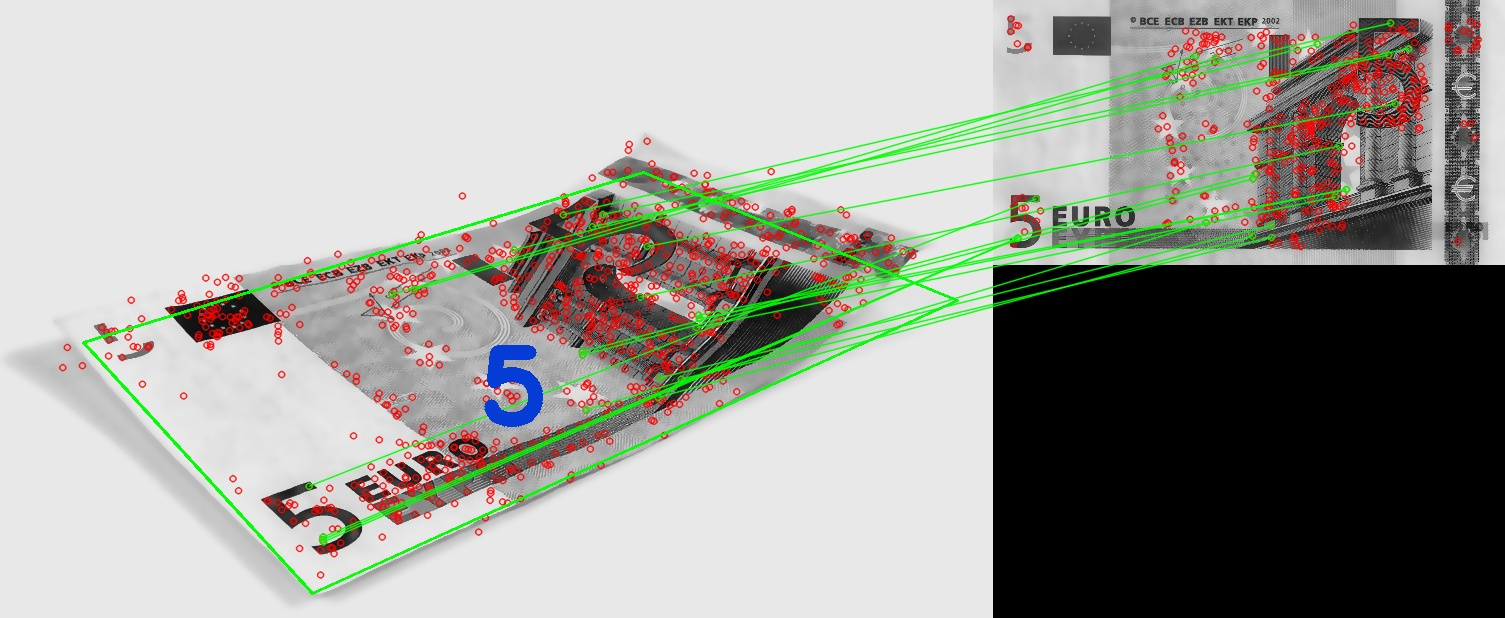
\includegraphics[width=0.82\textwidth]{notes-recognition/5__(6).jpg___SURF-Detector_SURF-Extractor_BF-Matcher_lowQualityImageDB_globalMatch__inliersMatches__0}
	\caption{Detection of a banknote with perspective distortion (using SURF detector, SURF descriptors and BFMatcher)}
	\label{fig:recognition-perspective-distortion}
\end{figure}

\begin{figure}[H]
	\centering
	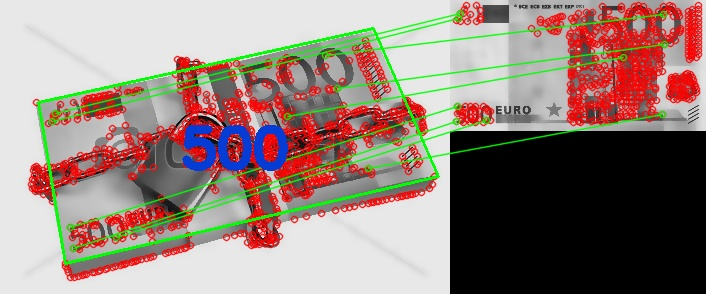
\includegraphics[width=0.498\textwidth]{notes-recognition/500.jpg___GFTT-Detector_SIFT-Extractor_BF-Matcher_dynamicQualityImageDB_globalMatch__inliersMatches__0}\hfill
	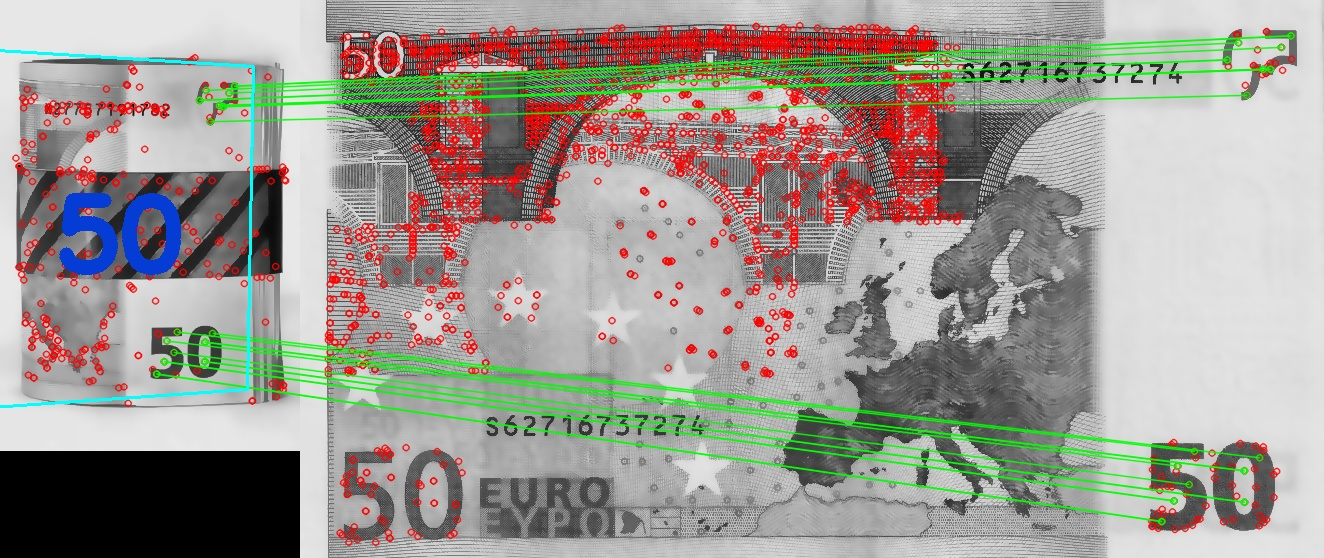
\includegraphics[width=0.498\textwidth]{notes-recognition/50__(13).jpg___SIFT-Detector_SIFT-Extractor_BF-Matcher_mediumQualityImageDB_globalMatch__inliersMatches__0}
	\caption{Detection of partially occluded banknotes (left image used GFTT detector, SIFT descriptors and BFMatcher while the right image used SIFT detector, SIFT descriptors and BFMatcher)}
	\label{fig:recognition-partially-occluded-banknotes}
\end{figure}

\begin{figure}[H]
	\centering
	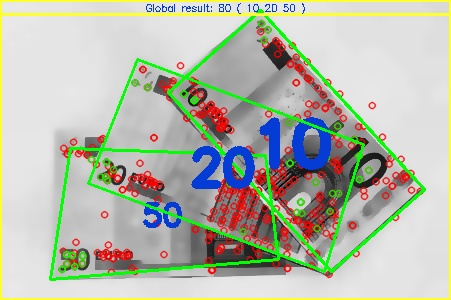
\includegraphics[width=0.498\textwidth]{notes-recognition/10-20-50.jpg___SIFT-Detector_SIFT-Extractor_BF-Matcher_dynamicQualityImageDB_globalMatch}\hfill
	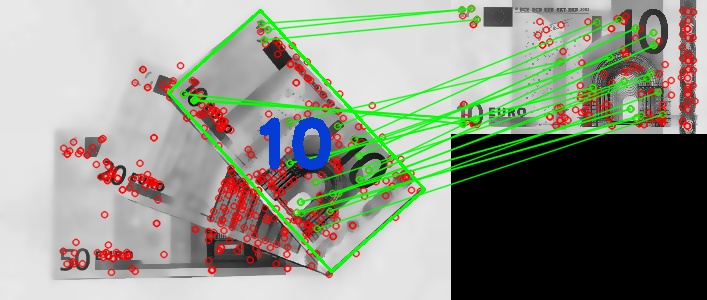
\includegraphics[width=0.498\textwidth]{notes-recognition/10-20-50.jpg___SIFT-Detector_SIFT-Extractor_BF-Matcher_dynamicQualityImageDB_globalMatch__inliersMatches__1}\hfill
	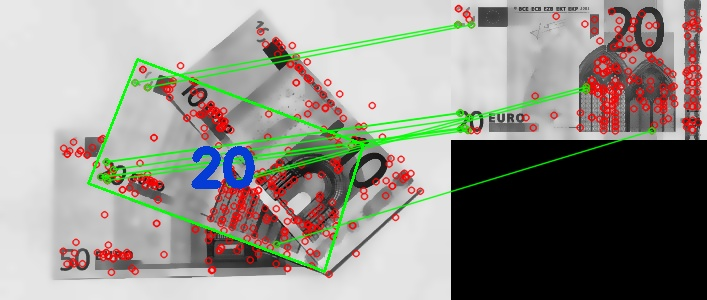
\includegraphics[width=0.498\textwidth]{notes-recognition/10-20-50.jpg___SIFT-Detector_SIFT-Extractor_BF-Matcher_dynamicQualityImageDB_globalMatch__inliersMatches__2}\hfill
	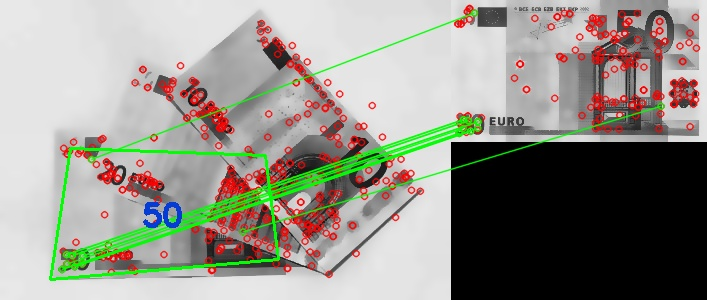
\includegraphics[width=0.498\textwidth]{notes-recognition/10-20-50.jpg___SIFT-Detector_SIFT-Extractor_BF-Matcher_dynamicQualityImageDB_globalMatch__inliersMatches__0}
	\caption{Detection of overlapping banknotes (using SIFT detector, SIFT descriptors and BFMatcher)}
	\label{fig:recognition-overlapping-banknotes}
\end{figure}
